% =====================================================================================================
%  MASTER COPY. Read EDIT_GUIDE.md before editing.
%    violet text  = sentences whose wording depends on the results, tagged [R1]..[R18] (EDIT_GUIDE.md §5)
%    blue [TODO]  = things to fill in that do not depend on results (EDIT_GUIDE.md §6)
%  Never type a result number into this file: add a key in fill_numbers.py and use \R{key}.
%  Camera-ready build: this file.  Double-blind build: main_blind.tex (no authors, no acknowledgment,
%  repository link withheld). Both read the same text.
% =====================================================================================================
\documentclass[conference]{IEEEtran}
\IEEEoverridecommandlockouts
\usepackage[T1]{fontenc}   % Times text in XeTeX/Tectonic builds too; harmless under pdfLaTeX (Overleaf)
\usepackage{cite}
\usepackage{amsmath,amssymb,amsfonts}
\usepackage{graphicx}
\usepackage{textcomp}
\usepackage{xcolor}
\usepackage{booktabs}
\usepackage{url}
\usepackage{tikz}
\usetikzlibrary{positioning,arrows.meta,calc}
\usepackage{pgfplots}
\pgfplotsset{compat=1.18}

% ---- result plumbing (do not edit) -------------------------------------------------------------------
\newif\iffinal
\finaltrue                       % <- \finalfalse shows result-dependent text in violet while editing
\newif\ifwatermark
\watermarkfalse
\newif\ifblind
\ifdefined\BLINDBUILD\blindtrue\else\blindfalse\fi   % set by main_blind.tex
\newif\ifplaceholderdata
\newcommand{\setR}[2]{\expandafter\def\csname R@#1\endcsname{#2}}
% AUTO-GENERATED by fill_numbers.py (--artifacts ..\results_0.5B) on 2026-10-09. Do not edit by hand.
\placeholderdatafalse
\setR{calib.bi.0.30.mark}{}
\setR{calib.bi.0.30.modes}{5.0}
\setR{calib.bi.0.30.multi}{100}
\setR{calib.bi.0.40.mark}{$\star$}
\setR{calib.bi.0.40.modes}{3.0}
\setR{calib.bi.0.40.multi}{90}
\setR{calib.bi.0.50.mark}{}
\setR{calib.bi.0.50.modes}{2.0}
\setR{calib.bi.0.50.multi}{60}
\setR{calib.bi.0.60.mark}{}
\setR{calib.bi.0.60.modes}{1.0}
\setR{calib.bi.0.60.multi}{35}
\setR{calib.bi.0.70.mark}{}
\setR{calib.bi.0.70.modes}{1.0}
\setR{calib.bi.0.70.multi}{5}
\setR{calib.emb.0.80.mark}{}
\setR{calib.emb.0.80.modes}{1.0}
\setR{calib.emb.0.80.multi}{2}
\setR{calib.emb.0.85.mark}{}
\setR{calib.emb.0.85.modes}{1.0}
\setR{calib.emb.0.85.multi}{12}
\setR{calib.emb.0.90.mark}{}
\setR{calib.emb.0.90.modes}{1.0}
\setR{calib.emb.0.90.multi}{48}
\setR{calib.emb.0.95.mark}{}
\setR{calib.emb.0.95.modes}{3.5}
\setR{calib.emb.0.95.multi}{88}
\setR{gsm.E1.bci}{--}
\setR{gsm.E1.est}{--}
\setR{gsm.E1.n}{--}
\setR{gsm.E1.p}{--}
\setR{gsm.E1.tci}{--}
\setR{gsm.E2.bci}{--}
\setR{gsm.E2.est}{--}
\setR{gsm.E2.n}{--}
\setR{gsm.E2.p}{--}
\setR{gsm.E2.tci}{--}
\setR{gsm.E3.bci}{--}
\setR{gsm.E3.est}{--}
\setR{gsm.E3.n}{--}
\setR{gsm.E3.p}{--}
\setR{gsm.E3.tci}{--}
\setR{gsm.P1.bci}{--}
\setR{gsm.P1.est}{--}
\setR{gsm.P1.n}{--}
\setR{gsm.P1.p}{--}
\setR{gsm.P1.sig}{--}
\setR{gsm.P1.tci}{--}
\setR{gsm.P2.bci}{--}
\setR{gsm.P2.est}{--}
\setR{gsm.P2.n}{--}
\setR{gsm.P2.p}{--}
\setR{gsm.P2.sig}{--}
\setR{gsm.P2.tci}{--}
\setR{gsm.S1.bci}{--}
\setR{gsm.S1.est}{--}
\setR{gsm.S1.n}{--}
\setR{gsm.S1.p}{--}
\setR{gsm.S1.tci}{--}
\setR{gsm.S2.bci}{--}
\setR{gsm.S2.est}{--}
\setR{gsm.S2.n}{--}
\setR{gsm.S2.p}{--}
\setR{gsm.S2.tci}{--}
\setR{gsm.S3.bci}{--}
\setR{gsm.S3.est}{--}
\setR{gsm.S3.n}{--}
\setR{gsm.S3.p}{--}
\setR{gsm.S3.tci}{--}
\setR{gsm.base.p1}{--}
\setR{gsm.base.p16}{--}
\setR{gsm.base.p2}{--}
\setR{gsm.base.p32}{--}
\setR{gsm.base.p4}{--}
\setR{gsm.base.p8}{--}
\setR{gsm.bbg.p1}{--}
\setR{gsm.bbg.p16}{--}
\setR{gsm.bbg.p2}{--}
\setR{gsm.bbg.p32}{--}
\setR{gsm.bbg.p4}{--}
\setR{gsm.bbg.p8}{--}
\setR{gsm.bbg.seeds}{--}
\setR{gsm.bbg.slope}{--}
\setR{gsm.cb.p1}{--}
\setR{gsm.cb.p16}{--}
\setR{gsm.cb.p2}{--}
\setR{gsm.cb.p32}{--}
\setR{gsm.cb.p4}{--}
\setR{gsm.cb.p8}{--}
\setR{gsm.cb.seeds}{--}
\setR{gsm.cb.slope}{--}
\setR{gsm.hcb.p1}{--}
\setR{gsm.hcb.p16}{--}
\setR{gsm.hcb.p2}{--}
\setR{gsm.hcb.p32}{--}
\setR{gsm.hcb.p4}{--}
\setR{gsm.hcb.p8}{--}
\setR{gsm.hcb.seeds}{--}
\setR{gsm.hcb.slope}{--}
\setR{gsm.heg.p1}{--}
\setR{gsm.heg.p16}{--}
\setR{gsm.heg.p2}{--}
\setR{gsm.heg.p32}{--}
\setR{gsm.heg.p4}{--}
\setR{gsm.heg.p8}{--}
\setR{gsm.heg.seeds}{--}
\setR{gsm.heg.slope}{--}
\setR{gsm.meg.p1}{--}
\setR{gsm.meg.p16}{--}
\setR{gsm.meg.p2}{--}
\setR{gsm.meg.p32}{--}
\setR{gsm.meg.p4}{--}
\setR{gsm.meg.p8}{--}
\setR{gsm.meg.seeds}{--}
\setR{gsm.meg.slope}{--}
\setR{gsm.rand.p1}{--}
\setR{gsm.rand.p16}{--}
\setR{gsm.rand.p2}{--}
\setR{gsm.rand.p32}{--}
\setR{gsm.rand.p4}{--}
\setR{gsm.rand.p8}{--}
\setR{gsm.rand.seeds}{--}
\setR{gsm.rand.slope}{--}
\setR{gsm.self.p1}{--}
\setR{gsm.self.p16}{--}
\setR{gsm.self.p2}{--}
\setR{gsm.self.p32}{--}
\setR{gsm.self.p4}{--}
\setR{gsm.self.p8}{--}
\setR{gsm.self.seeds}{--}
\setR{gsm.self.slope}{--}
\setR{gsm.vanilla.p1}{--}
\setR{gsm.vanilla.p16}{--}
\setR{gsm.vanilla.p2}{--}
\setR{gsm.vanilla.p32}{--}
\setR{gsm.vanilla.p4}{--}
\setR{gsm.vanilla.p8}{--}
\setR{gsm.vanilla.seeds}{--}
\setR{gsm.vanilla.slope}{--}
\setR{human.h1.A.acc}{53}
\setR{human.h1.A.same}{58}
\setR{human.h1.B.acc}{55}
\setR{human.h1.B.same}{51}
\setR{human.h1.acc}{55}
\setR{human.h1.alwayssame}{98}
\setR{human.h1.bacc}{77}
\setR{human.h1.cons.diff}{1}
\setR{human.h1.cons.same}{50}
\setR{human.h1.consensus}{51}
\setR{human.h1.items}{60}
\setR{human.h1.kappa}{0.13}
\setR{human.h1.pabak}{\ensuremath{+0.70}}
\setR{human.h1.rawagree}{85}
\setR{human.h2.A.exited}{7/20}
\setR{human.h2.A.p}{0.480}
\setR{human.h2.A.retained}{4/20}
\setR{human.h2.A.valid}{11}
\setR{human.h2.B.exited}{17/20}
\setR{human.h2.B.p}{0.082}
\setR{human.h2.B.retained}{11/20}
\setR{human.h2.B.valid}{28}
\setR{human.h2.consensus}{15}
\setR{human.h2.exited.ci}{[44, 97]}
\setR{human.h2.exited.n}{6}
\setR{human.h2.exited.rate}{83}
\setR{human.h2.exited.total}{20}
\setR{human.h2.items}{40}
\setR{human.h2.kappa}{-0.06}
\setR{human.h2.p}{0.041}
\setR{human.h2.pabak}{\ensuremath{-0.25}}
\setR{human.h2.rawagree}{38}
\setR{human.h2.retained.ci}{[6, 55]}
\setR{human.h2.retained.n}{9}
\setR{human.h2.retained.rate}{22}
\setR{math.E1.bci}{[\ensuremath{-0.91}, \ensuremath{+0.30}]}
\setR{math.E1.equiv}{yes}
\setR{math.E1.est}{\ensuremath{-0.31}}
\setR{math.E1.g32}{[\ensuremath{-3.2}, \ensuremath{+1.1}]}
\setR{math.E1.n}{3}
\setR{math.E1.p}{0.291}
\setR{math.E1.tci}{[\ensuremath{-0.92}, \ensuremath{+0.30}]}
\setR{math.E2.bci}{--}
\setR{math.E2.est}{--}
\setR{math.E2.n}{--}
\setR{math.E2.p}{--}
\setR{math.E2.tci}{--}
\setR{math.E3.bci}{--}
\setR{math.E3.est}{--}
\setR{math.E3.n}{--}
\setR{math.E3.p}{--}
\setR{math.E3.tci}{--}
\setR{math.P1.bci}{[\ensuremath{-0.79}, \ensuremath{+0.68}]}
\setR{math.P1.equiv}{yes}
\setR{math.P1.est}{\ensuremath{-0.02}}
\setR{math.P1.g32}{[\ensuremath{-2.7}, \ensuremath{+2.4}]}
\setR{math.P1.n}{3}
\setR{math.P1.p}{1.000}
\setR{math.P1.sig}{no}
\setR{math.P1.tci}{[\ensuremath{-1.13}, \ensuremath{+1.08}]}
\setR{math.P2.bci}{[\ensuremath{-0.60}, \ensuremath{+1.05}]}
\setR{math.P2.equiv}{yes}
\setR{math.P2.est}{\ensuremath{+0.22}}
\setR{math.P2.g32}{[\ensuremath{-2.1}, \ensuremath{+3.6}]}
\setR{math.P2.n}{3}
\setR{math.P2.p}{1.000}
\setR{math.P2.sig}{no}
\setR{math.P2.tci}{[\ensuremath{-1.34}, \ensuremath{+1.79}]}
\setR{math.S1.bci}{[\ensuremath{-0.94}, \ensuremath{+1.69}]}
\setR{math.S1.equiv}{no}
\setR{math.S1.est}{\ensuremath{+0.38}}
\setR{math.S1.g32}{[\ensuremath{-3.2}, \ensuremath{+5.9}]}
\setR{math.S1.n}{2}
\setR{math.S1.p}{0.493}
\setR{math.S1.tci}{[\ensuremath{-7.60}, \ensuremath{+8.36}]}
\setR{math.S2.bci}{[\ensuremath{-0.71}, \ensuremath{+1.68}]}
\setR{math.S2.equiv}{no}
\setR{math.S2.est}{\ensuremath{+0.46}}
\setR{math.S2.g32}{[\ensuremath{-2.5}, \ensuremath{+5.8}]}
\setR{math.S2.n}{2}
\setR{math.S2.p}{0.396}
\setR{math.S2.tci}{[\ensuremath{-5.92}, \ensuremath{+6.84}]}
\setR{math.S3.bci}{[\ensuremath{-0.59}, \ensuremath{+0.25}]}
\setR{math.S3.equiv}{yes}
\setR{math.S3.est}{\ensuremath{-0.18}}
\setR{math.S3.g32}{[\ensuremath{-2.0}, \ensuremath{+0.9}]}
\setR{math.S3.n}{2}
\setR{math.S3.p}{0.360}
\setR{math.S3.tci}{[\ensuremath{-1.48}, \ensuremath{+1.13}]}
\setR{math.base.p1}{30.3}
\setR{math.base.p16}{66.3}
\setR{math.base.p2}{40.4}
\setR{math.base.p32}{73.0}
\setR{math.base.p4}{50.1}
\setR{math.base.p8}{58.8}
\setR{math.bbg.entered}{--}
\setR{math.bbg.entropy}{--}
\setR{math.bbg.exited}{--}
\setR{math.bbg.p1}{--}
\setR{math.bbg.p16}{--}
\setR{math.bbg.p2}{--}
\setR{math.bbg.p32}{--}
\setR{math.bbg.p4}{--}
\setR{math.bbg.p8}{--}
\setR{math.bbg.posw}{--}
\setR{math.bbg.seeds}{--}
\setR{math.bbg.slope}{--}
\setR{math.cb.entered}{34.0}
\setR{math.cb.entropy}{0.73}
\setR{math.cb.exited}{26.0}
\setR{math.cb.p1}{31.2}
\setR{math.cb.p16}{67.9}
\setR{math.cb.p2}{41.5}
\setR{math.cb.p32}{74.6}
\setR{math.cb.p4}{51.3}
\setR{math.cb.p8}{60.2}
\setR{math.cb.posw}{1.00}
\setR{math.cb.seeds}{2}
\setR{math.cb.slope}{\ensuremath{+0.21}}
\setR{math.cb.slopesd}{0.33}
\setR{math.hcb.entered}{32.3}
\setR{math.hcb.entropy}{0.69}
\setR{math.hcb.exited}{20.7}
\setR{math.hcb.p1}{31.4}
\setR{math.hcb.p16}{68.5}
\setR{math.hcb.p2}{41.7}
\setR{math.hcb.p32}{75.3}
\setR{math.hcb.p4}{51.6}
\setR{math.hcb.p8}{60.6}
\setR{math.hcb.posw}{0.33}
\setR{math.hcb.seeds}{3}
\setR{math.hcb.slope}{\ensuremath{+0.37}}
\setR{math.hcb.slopesd}{0.28}
\setR{math.heg.entered}{33.3}
\setR{math.heg.entropy}{0.73}
\setR{math.heg.exited}{25.0}
\setR{math.heg.p1}{30.8}
\setR{math.heg.p16}{68.1}
\setR{math.heg.p2}{41.3}
\setR{math.heg.p32}{74.7}
\setR{math.heg.p4}{51.3}
\setR{math.heg.p8}{60.3}
\setR{math.heg.posw}{1.00}
\setR{math.heg.seeds}{3}
\setR{math.heg.slope}{\ensuremath{+0.35}}
\setR{math.heg.slopesd}{0.25}
\setR{math.meg.entered}{30.7}
\setR{math.meg.entropy}{0.74}
\setR{math.meg.exited}{28.3}
\setR{math.meg.p1}{30.4}
\setR{math.meg.p16}{67.1}
\setR{math.meg.p2}{40.8}
\setR{math.meg.p32}{73.5}
\setR{math.meg.p4}{50.8}
\setR{math.meg.p8}{59.7}
\setR{math.meg.posw}{1.00}
\setR{math.meg.seeds}{3}
\setR{math.meg.slope}{\ensuremath{+0.13}}
\setR{math.meg.slopesd}{0.40}
\setR{math.rand.entered}{--}
\setR{math.rand.entropy}{--}
\setR{math.rand.exited}{--}
\setR{math.rand.p1}{--}
\setR{math.rand.p16}{--}
\setR{math.rand.p2}{--}
\setR{math.rand.p32}{--}
\setR{math.rand.p4}{--}
\setR{math.rand.p8}{--}
\setR{math.rand.posw}{--}
\setR{math.rand.seeds}{--}
\setR{math.rand.slope}{--}
\setR{math.self.entered}{36.5}
\setR{math.self.entropy}{0.72}
\setR{math.self.exited}{25.5}
\setR{math.self.p1}{30.8}
\setR{math.self.p16}{68.0}
\setR{math.self.p2}{41.1}
\setR{math.self.p32}{75.2}
\setR{math.self.p4}{51.1}
\setR{math.self.p8}{60.1}
\setR{math.self.posw}{0.29}
\setR{math.self.seeds}{2}
\setR{math.self.slope}{\ensuremath{+0.48}}
\setR{math.self.slopesd}{0.05}
\setR{math.vanilla.entered}{36.3}
\setR{math.vanilla.entropy}{0.75}
\setR{math.vanilla.exited}{25.0}
\setR{math.vanilla.p1}{30.4}
\setR{math.vanilla.p16}{68.4}
\setR{math.vanilla.p2}{40.9}
\setR{math.vanilla.p32}{75.3}
\setR{math.vanilla.p4}{51.1}
\setR{math.vanilla.p8}{60.4}
\setR{math.vanilla.posw}{1.00}
\setR{math.vanilla.seeds}{3}
\setR{math.vanilla.slope}{\ensuremath{+0.66}}
\setR{math.vanilla.slopesd}{0.04}
\setR{mech.base.modes}{6.73}
\setR{mech.base.top}{43}
\setR{mech.cb.modes}{7.08}
\setR{mech.cb.top}{41}
\setR{mech.conc_exits.n}{16}
\setR{mech.conc_exits.p}{0.07}
\setR{mech.conc_exits.padj}{0.24}
\setR{mech.conc_exits.rho}{\ensuremath{-0.47}}
\setR{mech.div_exits.n}{16}
\setR{mech.div_exits.p}{0.02}
\setR{mech.div_exits.padj}{0.16}
\setR{mech.div_exits.rho}{\ensuremath{+0.57}}
\setR{mech.div_slope.n}{16}
\setR{mech.div_slope.p}{0.97}
\setR{mech.div_slope.padj}{0.97}
\setR{mech.div_slope.rho}{\ensuremath{-0.01}}
\setR{mech.ent_slope.n}{16}
\setR{mech.ent_slope.p}{0.67}
\setR{mech.ent_slope.padj}{0.94}
\setR{mech.ent_slope.rho}{\ensuremath{+0.11}}
\setR{mech.exits_slope.n}{16}
\setR{mech.exits_slope.p}{0.17}
\setR{mech.exits_slope.padj}{0.40}
\setR{mech.exits_slope.rho}{\ensuremath{-0.36}}
\setR{mech.hcb.modes}{6.70}
\setR{mech.hcb.top}{44}
\setR{mech.heg.modes}{6.98}
\setR{mech.heg.top}{41}
\setR{mech.kl_slope.n}{16}
\setR{mech.kl_slope.p}{0.26}
\setR{mech.kl_slope.padj}{0.46}
\setR{mech.kl_slope.rho}{\ensuremath{+0.30}}
\setR{mech.meg.modes}{7.55}
\setR{mech.meg.top}{38}
\setR{mech.nlinks}{7}
\setR{mech.self.modes}{6.97}
\setR{mech.self.top}{42}
\setR{mech.topic.n}{28}
\setR{mech.topic.p}{0.96}
\setR{mech.topic.padj}{0.97}
\setR{mech.topic.rho}{\ensuremath{+0.01}}
\setR{mech.vanilla.modes}{7.39}
\setR{mech.vanilla.top}{39}
\setR{meta.calib.basecor}{38}
\setR{meta.calib.modes}{3.0}
\setR{meta.calib.multishare}{90}
\setR{meta.crossk}{>32}
\setR{meta.entropy0}{0.63}
\setR{meta.epochs}{0.26}
\setR{meta.gpuh}{86}
\setR{meta.levels}{1--5}
\setR{meta.lr}{\ensuremath{1\times10^{-5}}}
\setR{meta.nseeds}{3}
\setR{meta.partitioner}{word-bigram Jaccard, threshold 0.4}
\setR{meta.rpp}{2.0}
\setR{meta.selrate}{59}
\setR{meta.sesoi}{1.0}
\setR{meta.sesoi32}{3.5}
\setR{meta.steps}{120}
\setR{meta.trainh}{48}
\setR{meta.usd}{87}
\setR{pow.E1.hw3}{0.61}
\setR{pow.E1.hw5}{0.31}
\setR{pow.E1.mde3}{0.8}
\setR{pow.E1.mde3pts}{2.6}
\setR{pow.E1.mde5}{0.4}
\setR{pow.E1.mde5pts}{1.4}
\setR{pow.E1.sd}{0.25}
\setR{pow.P1.hw3}{1.11}
\setR{pow.P1.hw5}{0.55}
\setR{pow.P1.mde3}{1.4}
\setR{pow.P1.mde3pts}{4.8}
\setR{pow.P1.mde5}{0.7}
\setR{pow.P1.mde5pts}{2.6}
\setR{pow.P1.sd}{0.45}
\setR{pow.P2.hw3}{1.57}
\setR{pow.P2.hw5}{0.78}
\setR{pow.P2.mde3}{2.0}
\setR{pow.P2.mde3pts}{6.8}
\setR{pow.P2.mde5}{1.0}
\setR{pow.P2.mde5pts}{3.6}
\setR{pow.P2.sd}{0.63}
\setR{pow.S1.hw3}{2.21}
\setR{pow.S1.hw5}{1.10}
\setR{pow.S1.mde3}{2.8}
\setR{pow.S1.mde3pts}{9.5}
\setR{pow.S1.mde5}{1.5}
\setR{pow.S1.mde5pts}{5.1}
\setR{pow.S1.sd}{0.89}
\setR{pow.S2.hw3}{1.76}
\setR{pow.S2.hw5}{0.88}
\setR{pow.S2.mde3}{2.2}
\setR{pow.S2.mde3pts}{7.6}
\setR{pow.S2.mde5}{1.2}
\setR{pow.S2.mde5pts}{4.1}
\setR{pow.S2.sd}{0.71}
\setR{pow.S3.hw3}{0.36}
\setR{pow.S3.hw5}{0.18}
\setR{pow.S3.mde3}{0.4}
\setR{pow.S3.mde3pts}{1.6}
\setR{pow.S3.mde5}{0.2}
\setR{pow.S3.mde5pts}{0.8}
\setR{pow.S3.sd}{0.15}
\setR{subj.alg.cb}{--}
\setR{subj.alg.heg}{--}
\setR{subj.alg.meg}{--}
\setR{subj.alg.vanilla}{--}
\setR{subj.cp.cb}{--}
\setR{subj.cp.heg}{--}
\setR{subj.cp.meg}{--}
\setR{subj.cp.vanilla}{--}
\setR{subj.geo.cb}{--}
\setR{subj.geo.heg}{--}
\setR{subj.geo.meg}{--}
\setR{subj.geo.vanilla}{--}
\setR{subj.ia.cb}{--}
\setR{subj.ia.heg}{--}
\setR{subj.ia.meg}{--}
\setR{subj.ia.vanilla}{--}
\setR{subj.nt.cb}{--}
\setR{subj.nt.heg}{--}
\setR{subj.nt.meg}{--}
\setR{subj.nt.vanilla}{--}
\setR{subj.pa.cb}{--}
\setR{subj.pa.heg}{--}
\setR{subj.pa.meg}{--}
\setR{subj.pa.vanilla}{--}
\setR{subj.pc.cb}{--}
\setR{subj.pc.heg}{--}
\setR{subj.pc.meg}{--}
\setR{subj.pc.vanilla}{--}
                  % written by fill_numbers.py
\newcommand{\resstyle}[1]{\ifplaceholderdata\textcolor{red}{#1}\else#1\fi}
\newcommand{\R}[1]{\ifcsname R@#1\endcsname\resstyle{\csname R@#1\endcsname}\else
  \textbf{\textcolor{red}{??#1??}}\PackageWarning{paper}{Missing result key #1}\fi}
\newcommand{\RT}[2]{\iffinal#2\else{\color{violet}#2\textsuperscript{\,[#1]}}\fi}
\newcommand{\TODO}[1]{\iffinal\errmessage{Unresolved TODO: #1}\else{\color{blue}[\textbf{TODO:} #1]}\fi}
\iffinal\ifplaceholderdata\errmessage{numbers.tex holds placeholder data: run fill_numbers.py --artifacts}\fi\fi
\ifplaceholderdata\ifwatermark
  \usepackage{draftwatermark}    % only while numbers.tex holds expected (not measured) values
  \SetWatermarkText{PLACEHOLDER RESULTS}
  \SetWatermarkScale{0.5}
  \SetWatermarkLightness{0.92}
\fi\fi

% ---- design constants (change here only if the pre-registration changes; see EDIT_GUIDE.md §8) -------
\newcommand{\cbTheta}{1.1}
\newcommand{\cbDelta}{0.18}
\newcommand{\cbEta}{0.05}
\newcommand{\megAlpha}{0.8}

\newcommand{\cond}[1]{\textsc{#1}}
\newcommand{\Ahat}{\hat{A}}
\newcommand{\Atil}{\tilde{A}}
\newcommand{\repo}{\ifblind an anonymized repository (link withheld for review)\else
  \url{https://github.com/2005legend/Reasoning-boundary-paradox-of-SLM}\fi}

\begin{document}
\bstctlcite{IEEEexample:BSTcontrol}

\title{Do Macro and Micro RLVR Interventions Compose?\\
A Pre-Registered Factorial Study of Reasoning Breadth and\\Solution Diversity in a Small Language Model}

\ifblind
\author{\IEEEauthorblockN{Anonymous Authors}\IEEEauthorblockA{Paper under double-blind review}}
\else
\author{%
\IEEEauthorblockN{\textbf{Sidaarth Krishnakanth}}
\IEEEauthorblockA{Department of Computer Science\\and Engineering\\
Sathyabama Institute of\\Science and Technology\\
Chennai, India\\
{\scriptsize Email: ksidaarth2005@gmail.com}}
\and
\IEEEauthorblockN{\textbf{Shivam Sunderam}}
\IEEEauthorblockA{Department of Computer Science\\and Engineering\\
Sathyabama Institute of\\Science and Technology\\
Chennai, India\\
{\scriptsize Email: shivamsunderam.cse@gmail.com}}
\and
\IEEEauthorblockN{\textbf{Ms.\ T.\ Bhanu Shree}}
\IEEEauthorblockA{Department of Computer Science\\and Engineering\\
Sathyabama Institute of\\Science and Technology\\
Chennai, India\\
{\scriptsize Email: ubhanukrithik@gmail.com}}
}
\fi

\maketitle

\begin{abstract}
Reinforcement learning with verifiable rewards (RLVR) raises the single-sample accuracy of language models.
Whether it also shrinks the set of problems a model can solve is disputed: base models overtake RLVR-trained ones
at large $k$ in some studies, longer training expands the boundary in others, and a third line traces the decline
to how Pass@$k$ is measured. All of this evidence is automatic, nobody has asked people what RLVR loses, and fixes
that act within a rollout group and across prompts have never been tested together. We take up all three gaps on
Qwen2.5-0.5B-Instruct trained with GRPO on MATH. A pre-registered $2\times3$ factorial crosses a macro factor (none,
or a topic-level budget on positive advantage) with a micro factor (none, the per-prompt SELF filter, or
mean-preserving redistribution over solution modes), with two or three seeds per cell, and a blinded human audit
checks what is lost. At \R{meta.rpp} rollouts per training problem, \RT{R1}{vanilla GRPO does not shrink the
boundary. MATH-500 Pass@1 moves from \R{math.base.p1}\% to \R{math.vanilla.p1}\%, Pass@32 rises from
\R{math.base.p32}\% to \R{math.vanilla.p32}\%, and every condition gains more problems than it loses. Neither
pre-registered contrast is significant: under the budget, swapping the SELF filter for mode redistribution changes
the gain from $k=1$ to $k=32$ by \R{math.P1.g32} points (95\% CI), and adding the budget to the redistribution by
\R{math.P2.g32}.} \RT{R17}{The two annotators agreed on \R{human.h1.rawagree}\% of solution pairs (PABAK
\R{human.h1.pabak}) and judged \R{human.h1.cons.same} of the \R{human.h1.consensus} agreed pairs to use the same
approach. The word-overlap partitioner that splits such pairs into ``modes'' scores \R{human.h1.acc}\% against them,
below the \R{human.h1.alwayssame}\% of a labeller that always answers ``same''. The diversity these fixes reweight is
mostly wording. Labels of reasoning validity agreed no better than chance, so what was lost stays open.} We read the
null as a matter of training intensity, not model size. The protocol runs on one 24\,GB GPU and is released.
\end{abstract}

\begin{IEEEkeywords}
reinforcement learning with verifiable rewards, GRPO, Pass@$k$, reasoning boundary, small language
models, credit assignment, human evaluation, pre-registration
\end{IEEEkeywords}

% =====================================================================================================
\section{Introduction}
% =====================================================================================================
Group Relative Policy Optimization (GRPO)~\cite{shao2024deepseekmath} and related RLVR methods are now the
standard way to improve mathematical reasoning in open language models. Whether they teach a model to solve new
problems, or only to solve solvable ones more reliably, is disputed. Yue et al.~\cite{yue2025rl} found that base
models overtake their RLVR-trained versions when many samples are drawn, a \emph{Pass@$k$ inversion} later analysed
as a shrinking reasoning boundary~\cite{nguyen2025paradox,zhou2026inversion,wu2025leash,zhou2026entrance}. Others
report the opposite. Prolonged training expands the boundary~\cite{liu2025prorl}, RLVR comes out ahead when only
correct chains of thought are counted~\cite{wen2025implicit}, and a two-stage account reconciles the two by training
duration~\cite{yao2025debate}. A third view blames the measurement: aggregate declines track how few rollouts each
training problem receives~\cite{yuan2026overtraining}, and Pass@$k$ at large $k$ rewards lucky
hits~\cite{dragoi2025breadth}. The question matters most for small language models (SLMs), which depend on
sampling-based coverage such as majority voting and verifier reranking.

The evidence on every side is automatic. Pass@$k$ cannot tell a valid solution from a lucky guess. CoT-Pass@$k$
hands that judgment to LLM judges, which accept corrupted reasoning almost as often as clean
reasoning~\cite{tasalti2026cotaudit}, and approach-level diversity has been scored by an LLM judge calibrated on 80
human-labelled pairs~\cite{lee2026strategy}. As far as we know, no study has asked people what RLVR loses: whether
the solutions that disappear are distinct strategies, and whether lost problems were ever solved by valid reasoning.

A third gap concerns the fixes. \emph{Intra-group} methods give rare correct modes of one prompt more credit than
common ones~\cite{cao2026cuegrpo,park2026reco,chen2026gcpo,chen2025dragrpo,liu2026edas,cao2026treeadv}, and
\emph{cross-prompt} methods reweight whole problems or
tasks~\cite{sun2026curverl,yuan2026overtraining,ramesh2026mtgrpo,nguyen2025paradox}. The two act on different axes
but have not been tested together (ReCo combines two corrections, both within one prompt~\cite{park2026reco}). One
pre-registered study addresses all three gaps:
\begin{itemize}
\item \emph{Is shrinkage real at SLM scale?} A multi-seed measurement on Qwen2.5-0.5B-Instruct~\cite{qwen2024qwen25}
trained on MATH~\cite{hendrycks2021math}, with problem-level boundary entries and exits and the number of rollouts
per training problem~\cite{yuan2026overtraining}.
\item \emph{What is lost, according to people?} A blinded audit of (H1) whether our partitioner's solution modes
are distinct strategies and (H2) whether the base model's successes on lost problems were valid reasoning.
\item \emph{Do the fixes compose?} A $2\times3$ factorial crossing a topic-level budget on positive advantage (CB,
macro) with no micro term, the SELF filter, or intra-group mode-rarity redistribution (MEG).
\item \RT{R2}{The answers: at about two rollouts per training problem RLVR expands the boundary slightly, no fix or
combination moves the shrinkage slope by more than about one point per unit $\ln k$, and the modes the fixes rely
on are mostly wording.}
\end{itemize}

% =====================================================================================================
\section{Related Work}
% =====================================================================================================
\textbf{Is shrinkage real?} Yue et al.~\cite{yue2025rl} showed that base models overtake RLVR-trained ones at large
$k$. Nguyen et al.~\cite{nguyen2025paradox} attribute this to negative interference and winner-take-all
reinforcement and propose SELF, which trains only on problems whose greedy answer is wrong. Wu and
Xuan~\cite{wu2025leash} argue that RLVR cannot leave the base model's support, Zhou and Li~\cite{zhou2026entrance}
place the contraction at the first decision of a solution, and Zhou~\cite{zhou2026inversion} diagnoses the
inversion. Against this, ProRL~\cite{liu2025prorl} reports expansion after prolonged, KL-controlled training, Wen et
al.~\cite{wen2025implicit} report expansion under CoT-Pass@$k$, and Yao et al.~\cite{yao2025debate} describe an
exploitation stage that shrinks the boundary followed by an exploration stage that expands it. Yuan et
al.~\cite{yuan2026overtraining} tie the decline to rollouts per problem and gate problems by success count (BBG),
and Dragoi et al.~\cite{dragoi2025breadth} show that Pass@$k$ favours lucky hits. Other work changes the optimizer
or the search~\cite{ba2026es,yu2026datpo,decugis2026fade}. At SLM scale, GRPO dynamics~\cite{ghosh2026dynamics},
difficulty scaling~\cite{yadav2026difficulty} and reward granularity~\cite{palandye2026granularity} have been
studied, but not shrinkage.

\textbf{Measuring what is lost.} Lee et al.~\cite{lee2026strategy} find that embedding similarity tracks phrasing
more than strategy and word-bigram overlap tracks approach better, and that 0.7\% of GSM8K problems but 33\% of MATH
problems admit more than one approach. Yang et al.~\cite{yang2026strategy} code the strategies of frontier models
with AI coders and human adjudication, without RL. Ta\c{s}alt{\i} et al.~\cite{tasalti2026cotaudit} find that
CoT-Pass@$k$ judges accept corrupted chains, and that Pass@$k$ exceeds CoT-Pass@$k$ by 19.7 points on
Qwen2.5-generation solvers. Our audit puts people directly on RLVR outcomes.

\textbf{Intra-group credit redistribution.} Cue-GRPO~\cite{cao2026cuegrpo} redistributes positive credit over a
partition of the correct rollouts by rarity and restores the mean; we adopt its rule as our micro term.
ReCo~\cite{park2026reco} reweights against concentration at the response and token level, and
GCPO~\cite{chen2026gcpo}, DRA-GRPO~\cite{chen2025dragrpo}, EDAS~\cite{liu2026edas} and TreeAdv~\cite{cao2026treeadv}
reshape advantages using diversity or structure within the group.

\textbf{Cross-prompt reweighting.} MT-GRPO~\cite{ramesh2026mtgrpo} reweights explicit tasks for worst-task
reliability, CurveRL~\cite{sun2026curverl} reweights prompts by pass-rate distribution, BBG gates problems by success
count~\cite{yuan2026overtraining}, and SELF selects by greedy failure~\cite{nguyen2025paradox}. CB works at the level
of topics, uses each topic's share of positive advantage as its signal, and keeps state across steps. We ask whether
a topic-level and an intra-group intervention compose, not which gate is best.

% =====================================================================================================
\section{Method}
% =====================================================================================================
\subsection{GRPO with gated advantages}
For a prompt $x$ the policy $\pi_\theta$ samples $G$ completions $y_1,\dots,y_G$ with binary rewards
$r_i\in\{0,1\}$. GRPO~\cite{shao2024deepseekmath} uses the group-normalized advantage
$\Ahat_i = (r_i-\operatorname{mean}(r))/(\operatorname{std}(r)+\epsilon)$. Every condition multiplies it by a
non-negative gate weight, $\Atil_i = g_i\,\Ahat_i$ with $g_i = g^{\mathrm{mac}}_i\, g^{\mathrm{mic}}_i$, and minimizes
the PPO-clip loss~\cite{schulman2017ppo} averaged over all $T$ completion tokens in the batch~\cite{yu2025dapo}:
\begin{equation}
\mathcal{L}(\theta) = -\frac{1}{T}\sum_{i}\sum_{t=1}^{|y_i|}
\min\!\big(\rho_{i,t}\Atil_i,\ \operatorname{clip}(\rho_{i,t},1-\varepsilon,1+\varepsilon)\,\Atil_i\big),
\label{eq:loss}
\end{equation}
where $\rho_{i,t}$ is the token probability ratio. Updates are on-policy with no KL penalty, and vanilla GRPO is
$g_i\equiv1$. Fig.~\ref{fig:method} shows one training step.

\begin{figure*}[t]
\centering
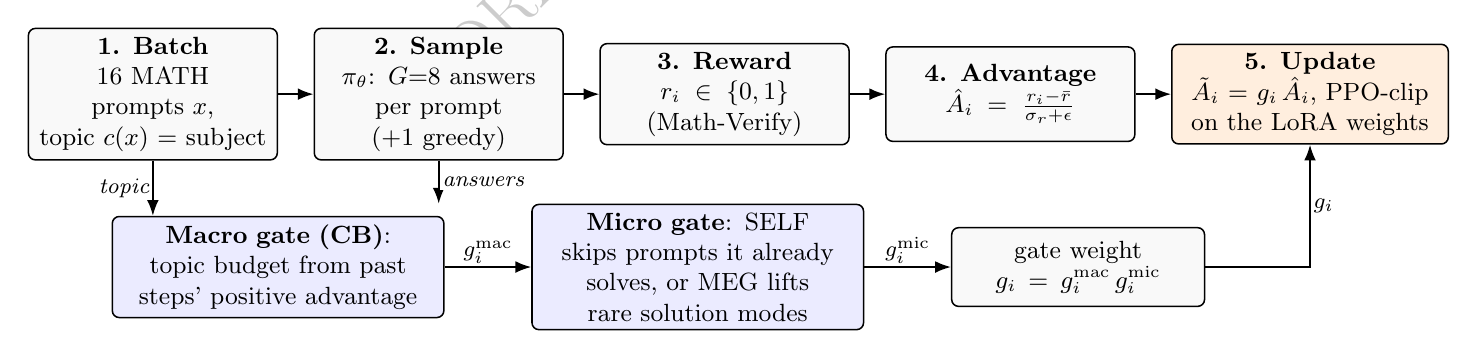
\begin{tikzpicture}[font=\small, node distance=5mm and 4.5mm,
  box/.style={draw, rounded corners=2.5pt, align=center, inner sep=3pt, text width=2.95cm, minimum height=12mm,
              line width=0.55pt, fill=gray!5},
  gate/.style={box, fill=blue!8, text width=4.0cm},
  upd/.style={box, fill=orange!13, text width=3.3cm},
  arr/.style={-{Latex[length=2mm]}, line width=0.65pt},
  lab/.style={font=\footnotesize\itshape, fill=white, inner sep=1pt}]
\node[box] (x) {\textbf{1. Batch}\\ 16 MATH prompts $x$,\\ topic $c(x)$ = subject};
\node[box, right=of x] (pi) {\textbf{2. Sample}\\ $\pi_\theta$: $G{=}8$ answers\\ per prompt (+1 greedy)};
\node[box, right=of pi] (r) {\textbf{3. Reward}\\ $r_i\in\{0,1\}$\\ (Math-Verify)};
\node[box, right=of r] (adv) {\textbf{4. Advantage}\\ $\Ahat_i=\frac{r_i-\bar r}{\sigma_r+\epsilon}$};
\node[upd, right=of adv] (u) {\textbf{5. Update}\\ $\Atil_i = g_i\,\Ahat_i$, PPO-clip\\ on the LoRA weights};
\node[gate, below=7mm of x.south east, anchor=north] (mac)
  {\textbf{Macro gate (CB)}: topic budget from past steps' positive advantage};
\node[gate, right=11mm of mac] (mic)
  {\textbf{Micro gate}: SELF skips prompts it already solves, or MEG lifts rare solution modes};
\node[box, right=11mm of mic, text width=3.0cm, minimum height=10mm] (g)
  {gate weight\\ $g_i = g^{\mathrm{mac}}_i\, g^{\mathrm{mic}}_i$};
\draw[arr] (x) -- (pi);
\draw[arr] (pi) -- (r);
\draw[arr] (r) -- (adv);
\draw[arr] (adv) -- (u);
\draw[arr] (x.south) -- node[lab, left] {topic} (x.south |- mac.north);
\draw[arr] (pi.south) -- node[lab, right] {answers} (pi.south |- mic.north);
\draw[arr] (mac) -- node[lab, above] {$g^{\mathrm{mac}}_i$} (mic);
\draw[arr] (mic) -- node[lab, above] {$g^{\mathrm{mic}}_i$} (g);
\draw[arr] (g.east) -| node[lab, pos=0.75, right] {$g_i$} (u.south);
\end{tikzpicture}
\caption{One training step of gated GRPO. The macro gate knows each prompt's topic and how much positive advantage
that topic has absorbed in past steps; the micro gate sees the current group's answers (and greedy answer). Their
product scales the advantage. Vanilla GRPO sets both gates to 1.}
\label{fig:method}
\end{figure*}

\subsection{Macro gate: topic budget (CB)}
Topics are the $C=7$ MATH subjects. After each step CB updates an exponential moving average of each topic's
\emph{spend}, the mean positive advantage of its rollouts in that step:
$s_c \leftarrow (1-\eta)\,s_c + \eta\,\operatorname{mean}_{i:c(x_i)=c}\max(\Ahat_i,0)$ with $\eta=\cbEta$. Negative
advantage never uses up a topic's budget. With the overspend ratio $\rho_c = s_c / \tfrac{1}{C}\sum_{c'} s_{c'}$,
\begin{equation}
\tilde g_c = \delta^{\max(0,\ \rho_c-\vartheta)},\qquad \vartheta=\cbTheta,\ \delta=\cbDelta ,
\label{eq:cb}
\end{equation}
so a topic at $1.5\times$ the average spend gets half the credit of one within budget. The gate acts only on
rollouts with positive advantage; their weights are clipped to $[0.3,3]$ and rescaled to mean 1 over the step, so
CB moves credit between topics instead of lowering the learning rate. The original specification ($\vartheta=1.5$,
$\delta=0.98$, down-weighting only) never fired in the pilot, where spend ratios stayed within $[0.38,1.46]$, so we
changed it before any main run and recorded the change in the pre-registration.

\subsection{Micro gates: SELF filter and mode redistribution (MEG)}
\textbf{SELF.} Following~\cite{nguyen2025paradox}, a prompt whose greedy answer is already correct gets weight
$\lambda=0$ and every other prompt weight 1. The greedy answer is decoded as one extra row of the same generation
call. We implement the selection rule only, not SELF's forward-KL term.

\textbf{MEG.} Let $\mathcal{C}$ be the $N$ correct rollouts of a group, partitioned into solution modes, and let
$|M(i)|$ be the size of the mode containing rollout $i$. Following Cue-GRPO~\cite{cao2026cuegrpo},
\begin{equation}
w_i = \frac{N\,|M(i)|^{-\alpha}}{\sum_{j\in\mathcal{C}}|M(j)|^{-\alpha}}\quad (i\in\mathcal{C}),\qquad
w_i = 1\quad (i\notin\mathcal{C}),
\label{eq:meg}
\end{equation}
with $\alpha=\megAlpha$, clipped to $[0.3,3]$ and rescaled to mean~1 over $\mathcal{C}$. MEG changes \emph{which}
correct solutions get credit, not how much; an earlier down-weight-only version was confounded with a lower
learning rate.

\textbf{Mode partitioner.} Modes come from agglomerative clustering of correct completions, on
MiniLM~\cite{wang2020minilm} sentence embeddings~\cite{reimers2019sbert} or on word-bigram Jaccard distance. A
pre-registered rule, applied to base-model rollouts before training, picks the candidate whose median number of modes
per group lies in $[2,4]$ and is closest to 3. It selected \R{meta.partitioner} (median \R{meta.calib.modes} modes,
\R{meta.calib.multishare}\% of groups with more than one; Table~\ref{tab:calib}). \RT{R15}{The embedding candidates
put almost every group's correct rollouts into a single mode}, which would make MEG a no-op.

\begin{table}[t]
\caption{Partitioner calibration on base-model rollouts (groups with $\ge4$ correct). $\star$ = selected.}
\label{tab:calib}
\centering\footnotesize
\setlength{\tabcolsep}{4pt}
\begin{tabular}{@{}lccccc@{}}
\toprule
MiniLM cosine $\tau$ & 0.80 & 0.85 & 0.90 & 0.95 & \\
\quad median modes & \R{calib.emb.0.80.modes}\R{calib.emb.0.80.mark} & \R{calib.emb.0.85.modes}\R{calib.emb.0.85.mark} & \R{calib.emb.0.90.modes}\R{calib.emb.0.90.mark} & \R{calib.emb.0.95.modes}\R{calib.emb.0.95.mark} & \\
\quad multi-mode groups (\%) & \R{calib.emb.0.80.multi} & \R{calib.emb.0.85.multi} & \R{calib.emb.0.90.multi} & \R{calib.emb.0.95.multi} & \\
\midrule
Word-bigram threshold & 0.30 & 0.40 & 0.50 & 0.60 & 0.70 \\
\quad median modes & \R{calib.bi.0.30.modes}\R{calib.bi.0.30.mark} & \R{calib.bi.0.40.modes}\R{calib.bi.0.40.mark} & \R{calib.bi.0.50.modes}\R{calib.bi.0.50.mark} & \R{calib.bi.0.60.modes}\R{calib.bi.0.60.mark} & \R{calib.bi.0.70.modes}\R{calib.bi.0.70.mark} \\
\quad multi-mode groups (\%) & \R{calib.bi.0.30.multi} & \R{calib.bi.0.40.multi} & \R{calib.bi.0.50.multi} & \R{calib.bi.0.60.multi} & \R{calib.bi.0.70.multi} \\
\bottomrule
\end{tabular}
\end{table}

\begin{table}[t]
\caption{The $2\times3$ factorial. Composites multiply the macro and micro gates.}
\label{tab:design}
\centering\footnotesize
\begin{tabular}{@{}lccc@{}}
\toprule
macro \textbackslash\ micro & none & SELF filter & MEG redistribution \\
\midrule
none & \cond{Vanilla} & \cond{SELF} & \cond{MEG} \\
CB topic budget & \cond{CB} & \cond{CB$\times$SELF} & \cond{CB$\times$MEG} (HEG-GRPO) \\
\bottomrule
\end{tabular}
\end{table}

% =====================================================================================================
\section{Experimental Setup}
% =====================================================================================================
\textbf{Training.} We train Qwen2.5-0.5B-Instruct~\cite{qwen2024qwen25} with LoRA~\cite{hu2021lora} adapters on the
MATH training split~\cite{hendrycks2021math} (7{,}496 problems with a boxed answer) under the standard ``reason step
by step and put the final answer in \texttt{\textbackslash boxed\{\}}'' prompt. Table~\ref{tab:design} lists the six
conditions and Table~\ref{tab:hparams} every setting. The reward is binary correctness checked with
Math-Verify~\cite{mathverify}, with a guarded symbolic fallback. The budget is \R{meta.epochs} epochs, or
\R{meta.rpp} rollouts per training problem. Seed $s$ fixes the data order and LoRA initialization across
conditions, so conditions are compared in seed-paired blocks.

\begin{table}[t]
\caption{Training and evaluation settings, the same for all conditions.}
\label{tab:hparams}
\centering\footnotesize
\begin{tabular}{@{}lp{0.70\columnwidth}@{}}
\toprule
Model & Qwen2.5-0.5B-Instruct, bf16; LoRA $r{=}16$, $\alpha{=}32$, all projections \\
Optimizer & AdamW, lr \R{meta.lr}, cosine, 10\% warm-up, grad-norm clip 1.0 \\
Batch, steps & 16 prompts $\times$ $G{=}8$ rollouts; \R{meta.steps} steps; MATH levels \R{meta.levels} \\
Sampling & $T{=}0.7$, top-$p$ 0.95, $\le$1{,}024 new tokens \\
Loss & PPO-clip $\varepsilon{=}0.2$, on-policy, token-level mean, no KL \\
CB / SELF / MEG & $\eta{=}\cbEta$, $\vartheta{=}\cbTheta$, $\delta{=}\cbDelta$ / $\lambda{=}0$ / $\alpha{=}\megAlpha$ \\
Evaluation & MATH-500, $n{=}32$ samples, $T{=}0.6$, top-$p$ 0.95 \\
Hardware & NVIDIA A10G 24\,GB (AWS g5.xlarge), one run per GPU \\
\bottomrule
\end{tabular}
\end{table}

\textbf{Evaluation and outcome.} Every model, including the base model, answers all of
MATH-500~\cite{lightman2023verify} 32 times per problem. Pass@$k$ for $k\in\{1,2,4,8,16,32\}$ uses the unbiased
estimator~\cite{chen2021codex}. MATH-500 shares no problem statement with the training split. The pre-registered
primary outcome is the \emph{shrinkage slope}, the least-squares slope of
$\Delta(k)=\text{Pass@}k(\text{run})-\text{Pass@}k(\text{base})$ against $\ln k$ in percentage points per unit
$\ln k$; a negative slope means gains at small $k$ turn into losses at large $k$. We also count boundary
\emph{exits} (problems the base model solves at least once in 32 samples and the trained model never does) and
\emph{entries} (the reverse).

\textbf{Pre-registered analysis.} Contrasts are linear combinations of condition slopes, paired by seed. The primary
contrasts are P1, \cond{CB$\times$MEG} $-$ \cond{CB$\times$SELF} (redistribution vs.\ filtering under the budget),
and P2, \cond{CB$\times$MEG} $-$ \cond{MEG} (does the macro level add to the micro level?). Secondary contrasts are
the two macro$\times$micro interactions (S1, S2), reported as bounds, and the macro main effect (S3); E1 is
exploratory. Each contrast has a hierarchical bootstrap interval over seeds and problems (2{,}000 resamples), and an
effect is claimed only if its Holm-adjusted~\cite{holm1979simple} $p<0.05$ and its interval excludes zero. The
pre-registration also fixed how outcomes are worded, including that a vanilla run without shrinkage is reported as
such.

\textbf{Human audit (pre-registered, secondary).} Two annotators who are not authors\ifblind\else, Shruti K (BBA)
and Sri Prathin (final-year B.E. CSE student)\fi, label two blinded sheets without seeing condition, group or
partitioner output. \emph{H1:} \R{human.h1.items} pairs of correct base-model solutions to the same training
problem, half placed in one mode by the partitioner and half in two, labelled \textsc{same} or \textsc{different}
approach under the definition of~\cite{lee2026strategy}; modes count as approach-level if the partitioner's balanced
accuracy against the consensus reaches 70\%. \emph{H2:} MATH-500 problems the base model solves but vanilla GRPO
never solves in a majority of seeds (\emph{exited}), each matched to a retained problem with the closest base solve
count. Annotators judge one correct base-model solution per problem \textsc{valid} or \textsc{flawed}, and the
groups are compared with a two-sided Fisher exact test.

\textbf{Reproducibility.} Code, logs, annotation sheets and the script behind every number are in \repo. The
pre-registration was written on 2026-10-03 and changed only by dated entries; it was first committed after the
runs\ifblind\else\ (\texttt{4cdc43a})\fi, so its dates are self-reported.

% =====================================================================================================
\section{Results}
% =====================================================================================================
\begin{table}[t]
\caption{MATH-500 Pass@$k$ (\%, mean over seeds), shrinkage slope (pp per unit $\ln k$; higher is better) and
boundary entries/exits (of 500 problems).}
\label{tab:main}
\centering\footnotesize
\setlength{\tabcolsep}{2.6pt}
\begin{tabular}{@{}lcccccc@{}}
\toprule
Condition & P@1 & P@4 & P@16 & P@32 & Slope & In / Out \\
\midrule
Base model & \R{math.base.p1} & \R{math.base.p4} & \R{math.base.p16} & \R{math.base.p32} & -- & -- \\
\cond{Vanilla} & \R{math.vanilla.p1} & \R{math.vanilla.p4} & \R{math.vanilla.p16} & \R{math.vanilla.p32} & \R{math.vanilla.slope} & \R{math.vanilla.entered} / \R{math.vanilla.exited} \\
\cond{SELF} & \R{math.self.p1} & \R{math.self.p4} & \R{math.self.p16} & \R{math.self.p32} & \R{math.self.slope} & \R{math.self.entered} / \R{math.self.exited} \\
\cond{MEG} & \R{math.meg.p1} & \R{math.meg.p4} & \R{math.meg.p16} & \R{math.meg.p32} & \R{math.meg.slope} & \R{math.meg.entered} / \R{math.meg.exited} \\
\cond{CB} & \R{math.cb.p1} & \R{math.cb.p4} & \R{math.cb.p16} & \R{math.cb.p32} & \R{math.cb.slope} & \R{math.cb.entered} / \R{math.cb.exited} \\
\cond{CB$\times$SELF} & \R{math.hcb.p1} & \R{math.hcb.p4} & \R{math.hcb.p16} & \R{math.hcb.p32} & \R{math.hcb.slope} & \R{math.hcb.entered} / \R{math.hcb.exited} \\
\cond{CB$\times$MEG} & \R{math.heg.p1} & \R{math.heg.p4} & \R{math.heg.p16} & \R{math.heg.p32} & \R{math.heg.slope} & \R{math.heg.entered} / \R{math.heg.exited} \\
\bottomrule
\end{tabular}
\end{table}

\begin{figure*}[t]
\centering
\pgfplotsset{every axis/.append style={font=\footnotesize, legend style={font=\scriptsize}},
  cv/.style={black, mark=*, mark size=1.3pt}, cs/.style={orange!85!black, mark=triangle*, mark size=1.6pt},
  cm/.style={teal, mark=square*, mark size=1.2pt}, cc/.style={gray, dashed, mark=o, mark size=1.3pt},
  ch/.style={brown!80!black, dashed, mark=triangle, mark size=1.6pt}, ce/.style={blue, very thick, mark=diamond*, mark size=2pt}}
\begin{minipage}[t]{0.49\textwidth}\centering
\begin{tikzpicture}
\begin{axis}[width=\linewidth, height=4.6cm, xmode=log, log basis x=2, xtick={1,2,4,8,16,32},
  xticklabels={1,2,4,8,16,32}, xlabel={$k$}, ylabel={$\Delta$Pass@$k$ vs.\ base (pp)},
  grid=major, grid style={gray!20}, legend columns=3, legend pos=north west,
  error bars/y dir=both, error bars/y explicit]
\addplot+[cv] table[x=k, y=vanilla, y error=vanilla_err] {figdata/delta_math.dat};
\addplot+[cs] table[x=k, y=self, y error=self_err] {figdata/delta_math.dat};
\addplot+[cm] table[x=k, y=meg, y error=meg_err] {figdata/delta_math.dat};
\addplot+[cc] table[x=k, y=cb, y error=cb_err] {figdata/delta_math.dat};
\addplot+[ch] table[x=k, y=hcb, y error=hcb_err] {figdata/delta_math.dat};
\addplot+[ce] table[x=k, y=heg, y error=heg_err] {figdata/delta_math.dat};
\draw[gray] (axis cs:1,0) -- (axis cs:32,0);
\legend{Vanilla, SELF, MEG, CB, CB$\times$SELF, CB$\times$MEG}
\end{axis}
\end{tikzpicture}
\end{minipage}\hfill
\begin{minipage}[t]{0.49\textwidth}\centering
\begin{tikzpicture}
\begin{axis}[width=\linewidth, height=4.6cm, xlabel={training step}, ylabel={mode entropy (normalized)},
  grid=major, grid style={gray!20}, legend columns=3, legend pos=south west]
\addplot+[cv, mark repeat=4] table[x=step, y=vanilla] {figdata/entropy.dat};
\addplot+[cs, mark repeat=4] table[x=step, y=self] {figdata/entropy.dat};
\addplot+[cm, mark repeat=4] table[x=step, y=meg] {figdata/entropy.dat};
\addplot+[cc, mark repeat=4] table[x=step, y=cb] {figdata/entropy.dat};
\addplot+[ch, mark repeat=4] table[x=step, y=hcb] {figdata/entropy.dat};
\addplot+[ce, mark repeat=4] table[x=step, y=heg] {figdata/entropy.dat};
\legend{Vanilla, SELF, MEG, CB, CB$\times$SELF, CB$\times$MEG}
\end{axis}
\end{tikzpicture}
\end{minipage}
\caption{Left: change in MATH-500 Pass@$k$ relative to the base model (mean $\pm$ s.d.\ over seeds); a curve that
fell below zero at large $k$ would mean a shrunk boundary. Right: normalized entropy of the solution-mode
distribution among correct rollouts during training (mean over seeds).}
\label{fig:curves}
\end{figure*}

\subsection{Shrinkage at 0.5B}
\RT{R3}{Vanilla GRPO does not reproduce the inversion at this budget.} Pass@1 moves from \R{math.base.p1}\% to
\R{math.vanilla.p1}\% and Pass@32 rises from \R{math.base.p32}\% to \R{math.vanilla.p32}\% (Table~\ref{tab:main}).
The curve stays above zero up to $k=32$, with slope \R{math.vanilla.slope} (Fig.~\ref{fig:curves}, left). On
average \R{math.vanilla.entered} problems enter the boundary and \R{math.vanilla.exited} leave it, and every other
condition also has a positive slope and more entries than exits. Each training problem received \R{meta.rpp}
rollouts on average, the low-visit end that SLM budgets allow; aggregate shrinkage has been tied to how often a
problem is revisited~\cite{yuan2026overtraining}.

\subsection{Pre-registered contrasts}
\begin{table}[t]
\caption{Contrasts on the MATH-500 shrinkage slope (pp per unit $\ln k$), paired by seed, with hierarchical
bootstrap CIs; the last column restates the CI as points of gain from $k{=}1$ to $k{=}32$. $p$: Holm-adjusted for
P1--P2.}
\label{tab:contrasts}
\centering\footnotesize
\setlength{\tabcolsep}{1.9pt}
\begin{tabular}{@{}llcccc@{}}
\toprule
 & Contrast & Est. & 95\% CI & $p$ & CI, $k{=}1{\to}32$ \\
\midrule
P1 & CB$\times$MEG $-$ CB$\times$SELF & \R{math.P1.est} & \R{math.P1.bci} & \R{math.P1.p} & \R{math.P1.g32} \\
P2 & CB$\times$MEG $-$ MEG & \R{math.P2.est} & \R{math.P2.bci} & \R{math.P2.p} & \R{math.P2.g32} \\
\midrule
S1 & CB$\times$MEG interaction & \R{math.S1.est} & \R{math.S1.bci} & \R{math.S1.p} & \R{math.S1.g32} \\
S2 & CB$\times$SELF interaction & \R{math.S2.est} & \R{math.S2.bci} & \R{math.S2.p} & \R{math.S2.g32} \\
S3 & CB main effect & \R{math.S3.est} & \R{math.S3.bci} & \R{math.S3.p} & \R{math.S3.g32} \\
\midrule
E1 & CB$\times$MEG $-$ Vanilla & \R{math.E1.est} & \R{math.E1.bci} & \R{math.E1.p} & \R{math.E1.g32} \\
\bottomrule
\end{tabular}
\end{table}

\RT{R4}{All six slopes are positive, from \R{math.meg.slope} (\cond{MEG}) to \R{math.vanilla.slope}
(\cond{Vanilla}), and no gate beats vanilla.} \RT{R5}{Neither primary contrast clears the pre-registered bar
(Table~\ref{tab:contrasts}).} \RT{R6}{In points of gain between $k=1$ and $k=32$, P1 lies within \R{math.P1.g32} and
P2 within \R{math.P2.g32}, so any difference between the micro terms is under about three points. The interactions
are wider, \R{math.S1.g32} and \R{math.S2.g32}, which admits effects larger than vanilla's whole gain at $k=32$; with
two seeds per cell the interaction question stays open.} \RT{R19}{Both primary 90\% intervals lie inside
$\pm\R{meta.sesoi}$ pp per $\ln k$ ($\pm\R{meta.sesoi32}$ points at $k=32$), so we call P1 and P2 equivalent to zero
within that bound, which we chose after seeing the data; the interactions do not meet it. With the between-seed
spread we observed, three seeds detect a difference of about \R{pow.P1.mde3} (P1) and \R{pow.P2.mde3} (P2) pp per
$\ln k$ at 80\% power, and five seeds would detect \R{pow.P1.mde5} and \R{pow.P2.mde5}.} We read the primary
contrasts as a bounded null, as pre-registered. The gates also made runs less reproducible: the slope's standard deviation across seeds is
\R{math.vanilla.slopesd} for \cond{Vanilla} and \R{math.meg.slopesd} for \cond{MEG} (\R{math.heg.slopesd} and
\R{math.hcb.slopesd} for the composites), a descriptive comparison at three seeds.

\subsection{What each level does}
Mode entropy of the correct rollouts starts at \R{meta.entropy0} and \RT{R7}{does not decay under vanilla GRPO}
(Fig.~\ref{fig:curves}, right). At evaluation, vanilla's correct answers to a problem fall into
\R{mech.vanilla.modes} modes on average, against \R{mech.base.modes} for the base model, and its largest mode holds
\R{mech.vanilla.top}\% of them against \R{mech.base.top}\%. There is no collapse for MEG to undo. \cond{SELF} skips
the \R{meta.selrate}\% of prompts it already solves, for a mean positive weight of \R{math.self.posw}. Changes are
uneven across subjects (Fig.~\ref{fig:subjects}): under vanilla GRPO, Pass@32 rises by \R{subj.cp.vanilla}~pp in
Counting \& Probability and by \R{subj.geo.vanilla}~pp in Geometry. \RT{R8}{The macro gate binds but changes
nothing. In the CB runs a subject's share of positive credit does not predict its Pass@32 change (Spearman
$\rho=\R{mech.topic.rho}$, $n=\R{mech.topic.n}$ subject-runs), which leaves the premise of a topic budget
unsupported.}

\begin{figure}[t]
\centering
\begin{tikzpicture}
\begin{axis}[ybar, bar width=2.3pt, width=\columnwidth, height=3.9cm, enlarge x limits=0.08,
  symbolic x coords={alg,cp,geo,ia,nt,pa,pc}, xtick=data,
  xticklabels={Alg., C\&P, Geom., Int.\,Alg., Num.\,Th., Prealg., Precalc.},
  tick label style={font=\scriptsize}, label style={font=\footnotesize}, ylabel={$\Delta$Pass@32 (pp)},
  ymajorgrids, grid style={gray!20}, legend columns=4,
  legend style={at={(0.5,1.03)}, anchor=south, font=\scriptsize, draw=none}]
\addplot[fill=black, draw=black] table[x=subj, y=vanilla] {figdata/subject_math.dat};
\addplot[fill=gray!55, draw=gray] table[x=subj, y=cb] {figdata/subject_math.dat};
\addplot[fill=teal!65, draw=teal] table[x=subj, y=meg] {figdata/subject_math.dat};
\addplot[fill=blue!80, draw=blue] table[x=subj, y=heg] {figdata/subject_math.dat};
\legend{Vanilla, CB, MEG, CB$\times$MEG}
\end{axis}
\end{tikzpicture}
\caption{Change in MATH-500 Pass@32 relative to the base model by subject, the macro gate's topics (mean over seeds).}
\label{fig:subjects}
\end{figure}

\RT{R9}{Boundary exits barely separate the conditions.} \cond{CB$\times$SELF} loses the fewest problems
(\R{math.hcb.exited}) and \cond{MEG} the most (\R{math.meg.exited}), against \R{math.vanilla.exited} for
\cond{Vanilla}. Across the \R{mech.div_exits.n} runs, those that gained more distinct correct modes lost slightly
more problems (Spearman $\rho=\R{mech.div_exits.rho}$, $p=\R{mech.div_exits.p}$), but this does not survive
correction over the \R{mech.nlinks} correlations we computed (Benjamini--Hochberg $p=\R{mech.div_exits.padj}$).
Since the next subsection shows these modes are mostly wording, we treat it as a hypothesis.

\subsection{What is lost: the human audit}
\textbf{H1, are the modes approaches?} \RT{R17}{The annotators called \R{human.h1.A.same} and \R{human.h1.B.same} of
the \R{human.h1.items} pairs the same approach, although the partitioner had split half of them. They agreed on
\R{human.h1.consensus} pairs (\R{human.h1.rawagree}\%), \R{human.h1.cons.same} \textsc{same} and
\R{human.h1.cons.diff} \textsc{different}. Cohen's $\kappa$ is only \R{human.h1.kappa} because almost every label
falls in one class, which depresses $\kappa$ however well raters agree; the prevalence-adjusted PABAK is
\R{human.h1.pabak}. Against the consensus the partitioner scores \R{human.h1.acc}\%, below the
\R{human.h1.alwayssame}\% of a labeller that always says \textsc{same}. The pre-registered balanced accuracy is
\R{human.h1.bacc}\%, formally above the 70\% bar, but one of its two classes holds a single pair, so we do not rely
on it. We read the modes as surface clusters, and MEG as redistributing credit over them.}

\textbf{H2, what is lost?} Despite its net gains, vanilla GRPO lost \R{human.h2.exited.total} problems in a majority
of seeds. \RT{R18}{The annotators disagreed on whether the base model's successes on them were valid: A rated
\R{human.h2.A.valid} of \R{human.h2.items} solutions valid and B \R{human.h2.B.valid} ($\kappa=\R{human.h2.kappa}$,
agreement on \R{human.h2.consensus} items). On those items, \R{human.h2.exited.rate}\% of exited solutions were valid
(CI \R{human.h2.exited.ci}, $n=\R{human.h2.exited.n}$) against \R{human.h2.retained.rate}\% of retained ones (CI
\R{human.h2.retained.ci}, $n=\R{human.h2.retained.n}$; Fisher $p=\R{human.h2.p}$). Read literally, the
pre-registered rule calls this a genuine loss, but a subset chosen by agreement at chance-level reliability cannot
carry that; each annotator alone shows the same direction without significance (A $p=\R{human.h2.A.p}$, B
$p=\R{human.h2.B.p}$).} We report H2 as inconclusive.

% =====================================================================================================
\section{Discussion and Limitations}
% =====================================================================================================
\RT{R13}{\textbf{Training intensity, not size.} With about two rollouts per training problem and a policy that moved
little (final KL to the base model about ten times its bf16 noise floor), RLVR on a 0.5B model expands the boundary
slightly. Accounts that tie shrinkage to repeated reinforcement of saturated problems~\cite{yuan2026overtraining} or
to a long exploitation phase~\cite{yao2025debate} predict exactly this, and the reported
inversions~\cite{yue2025rl,nguyen2025paradox} come from far longer training. We read our null as a statement about
the regime a single-GPU budget reaches, not about model size. It suggests a direct test: raise rollouts per problem
at 0.5B and shrinkage should appear. We have registered that test: five seeds per cell and 240-step runs scored at
steps 120, 180 and 240. Our prediction, made before running it, is that vanilla's slope declines over those steps;
if it does not, the intensity reading fails.} \textbf{The partition is the weak link.} Embedding partitions put nearly every
group in one mode (Table~\ref{tab:calib}), and the bigram partition finds about three modes that people see as one
approach. Neither tracks what intra-group methods assume it tracks, which matters for any method that reweights over
such partitions~\cite{cao2026cuegrpo,park2026reco,chen2026gcpo,chen2025dragrpo,liu2026edas}. This fits Lee et al.'s
finding that a third of MATH problems admit more than one approach~\cite{lee2026strategy}: the alternatives exist in
the dataset but rarely appear in what a 0.5B model samples. We do not claim that shrinkage is absent at larger
budgets; the bounds in Table~\ref{tab:contrasts} are what a longer study would need to beat.

\textbf{Limitations.} One model at one size, LoRA, one RL algorithm and short training (\R{meta.steps} steps, cut from
a planned 240), evaluated only on MATH-500. Two or three seeds per cell leave the interactions open, and each run has one full evaluation, so we show no
trajectory over training. SELF omits its
forward-KL term, and no random-partition control was run. The annotators differed in strictness on H2, and the
pre-registered third annotator was not used. The correlations above are descriptive and were added after the
pre-registration.

% =====================================================================================================
\section{Conclusion}
% =====================================================================================================
In a pre-registered study of Qwen2.5-0.5B-Instruct with a blinded human audit, \RT{R14}{shrinkage does not appear
at about two rollouts per training problem, and neither a topic-level budget, intra-group mode redistribution, nor
their combination moves the shrinkage slope by more than about one point per unit $\ln k$}. People judged the
partitioner's modes to be wording variants of one approach. The protocol runs on one 24\,GB GPU in
\R{meta.gpuh} GPU-hours and is released.

\ifblind\else
\section*{Acknowledgment}
We thank the two annotators. This work used AWS credits awarded to our team for placing among the top 500 teams in
the Amazon ML Challenge 2026; early experiments ran on a local NVIDIA RTX 3060 (12\,GB). AWS compute:
\R{meta.gpuh} A10G GPU-hours, about \$\R{meta.usd}. An AI assistant (Claude, Anthropic) was used to write analysis
code and to draft and edit parts of the text; the authors checked the results against the logs and take
responsibility for the content.
\fi

\bibliographystyle{IEEEtran}
\bibliography{IEEEabrv,refs}

\end{document}
